

\tikzset{every picture/.style={line width=0.75pt}} %set default line width to 0.75pt        

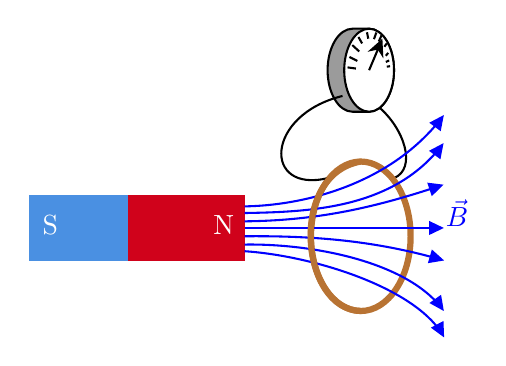
\begin{tikzpicture}[x=0.75pt,y=0.75pt,yscale=-1,xscale=1,scale=0.8]
%uncomment if require: \path (0,300); %set diagram left start at 0, and has height of 300

%Curve Lines [id:da6703211387696746] 
\draw    (290.63,57) .. controls (306.13,70) and (314,94) .. (300,100) ;


%Shape: Rectangle [id:dp8279373731612705] 
\draw  [draw opacity=0][fill={rgb, 255:red, 74; green, 144; blue, 226 }  ,fill opacity=1 ] (80,110) -- (140,110) -- (140,150) -- (80,150) -- cycle ;
%Shape: Rectangle [id:dp8107885000069281] 
\draw  [draw opacity=0][fill={rgb, 255:red, 208; green, 2; blue, 27 }  ,fill opacity=1 ] (140,110) -- (210,110) -- (210,150) -- (140,150) -- cycle ;
%Shape: Ellipse [id:dp5591787546303602] 
\draw  [color={rgb, 255:red, 184; green, 115; blue, 51 }  ,draw opacity=1 ][line width=2.25]  (250,135) .. controls (250,110.15) and (263.43,90) .. (280,90) .. controls (296.57,90) and (310,110.15) .. (310,135) .. controls (310,159.85) and (296.57,180) .. (280,180) .. controls (263.43,180) and (250,159.85) .. (250,135) -- cycle ;
%Shape: Path Data [id:dp12298055640296068] 
\draw  [fill={rgb, 255:red, 155; green, 155; blue, 155 }  ,fill opacity=1 ] (300,35) .. controls (300,48.81) and (293.28,60) .. (285,60) -- (275,60) .. controls (266.72,60) and (260,48.81) .. (260,35) .. controls (260,21.19) and (266.72,10) .. (275,10) -- (285,10) .. controls (293.28,10) and (300,21.19) .. (300,35) -- cycle ;
%Shape: Ellipse [id:dp5212685142947344] 
\draw  [fill={rgb, 255:red, 255; green, 255; blue, 255 }  ,fill opacity=1 ] (270,35) .. controls (270,21.19) and (276.72,10) .. (285,10) .. controls (293.28,10) and (300,21.19) .. (300,35) .. controls (300,48.81) and (293.28,60) .. (285,60) .. controls (276.72,60) and (270,48.81) .. (270,35) -- cycle ;

%Straight Lines [id:da5331302994346345] 
\draw    (285,35) -- (291.84,18.76) ;
\draw [shift={(293,16)}, rotate = 472.83] [fill={rgb, 255:red, 0; green, 0; blue, 0 }  ][line width=0.08]  [draw opacity=0] (10.72,-5.15) -- (0,0) -- (10.72,5.15) -- (7.12,0) -- cycle    ;

%Straight Lines [id:da47260473383861945] 
\draw    (272,33.29) -- (277.07,34) ;


%Straight Lines [id:da24575992815572056] 
\draw    (273.14,27) -- (277.93,29.43) ;


%Straight Lines [id:da39681633957826223] 
\draw    (274.86,19.86) -- (279.07,23.71) ;


%Straight Lines [id:da4645843525587261] 
\draw    (278.57,15) -- (280.79,18.86) ;


%Straight Lines [id:da8783682496108793] 
\draw    (283.71,12.14) -- (284.5,16) ;


%Straight Lines [id:da708942185389569] 
\draw    (289.36,12.29) -- (287.93,16.29) ;


%Straight Lines [id:da4987912734748998] 
\draw    (292.5,14) -- (290.79,17.71) ;


%Straight Lines [id:da9647680952785245] 
\draw    (295.64,18.86) -- (294.21,20.86) ;


%Straight Lines [id:da1204235998910006] 
\draw    (296.5,24.57) -- (295.07,26.29) ;


%Straight Lines [id:da824372964873956] 
\draw    (297.07,29.14) -- (295.07,30) ;


%Straight Lines [id:da3171407140640803] 
\draw    (297.64,32.57) -- (295.64,32.86) ;


%Curve Lines [id:da6638499736423984] 
\draw    (269,50.5) .. controls (222.13,62) and (220.8,109.32) .. (260,100) ;


%Curve Lines [id:da03143429830811484] 
\draw[blue]    (210,117) .. controls (249.2,116.35) and (298.72,102) .. (328.22,64.33) ;
\draw [shift={(330,62)}, rotate = 486.59,blue] [fill=blue  ][line width=0.08]  [draw opacity=0] (8.93,-4.29) -- (0,0) -- (8.93,4.29) -- cycle    ;

%Curve Lines [id:da1604140715333262] 
\draw[blue]    (210,144) .. controls (251.9,146.84) and (311.15,165.73) .. (328.66,193.33) ;
\draw [shift={(330.17,195.92)}, rotate = 242.13] [fill=blue][line width=0.08]  [draw opacity=0] (8.93,-4.29) -- (0,0) -- (8.93,4.29) -- cycle    ;

%Curve Lines [id:da10162390231110208] 
\draw[blue]    (210,121) .. controls (249.2,120.35) and (298.56,118.4) .. (328.05,81.24) ;
\draw[blue] [shift={(329.83,78.92)}, rotate = 486.59] [fill=blue][line width=0.08]  [draw opacity=0] (8.93,-4.29) -- (0,0) -- (8.93,4.29) -- cycle    ;

%Curve Lines [id:da1061280436537615] 
\draw[blue]    (210,140) .. controls (249,139.35) and (305.82,149.47) .. (328.34,177.79) ;
\draw[blue] [shift={(330,180)}, rotate = 234.69] [fill=blue][line width=0.08]  [draw opacity=0] (8.93,-4.29) -- (0,0) -- (8.93,4.29) -- cycle    ;

%Curve Lines [id:da6866149780262758] 
\draw[blue]    (210,126) .. controls (251.98,125.59) and (286.27,118.46) .. (327.31,104.76) ;
\draw[blue] [shift={(329.83,103.92)}, rotate = 521.3299999999999] [fill=blue][line width=0.08]  [draw opacity=0] (8.93,-4.29) -- (0,0) -- (8.93,4.29) -- cycle    ;

%Curve Lines [id:da4893977733064039] 
\draw[blue]    (210,135) .. controls (251.65,134.59) and (288.5,137.7) .. (327.76,148.89) ;
\draw[blue] [shift={(330.17,149.58)}, rotate = 196.31] [fill=blue][line width=0.08]  [draw opacity=0] (8.93,-4.29) -- (0,0) -- (8.93,4.29) -- cycle    ;

%Straight Lines [id:da933317715667781] 
\draw[blue]    (210,130) -- (327,130) ;
\draw[blue] [shift={(330,130)}, rotate = 180] [fill=blue][line width=0.08]  [draw opacity=0] (8.93,-4.29) -- (0,0) -- (8.93,4.29) -- cycle    ;

%Curve Lines [id:da500101752265627] 
\draw [color={rgb, 255:red, 184; green, 115; blue, 51 }  ,draw opacity=1 ][line width=2.25]    (280,90) .. controls (236,97.6) and (243.6,179.2) .. (280,180) ;


% Text Node
\draw (93,128.5) node [color={rgb, 255:red, 255; green, 255; blue, 255 }  ,opacity=1 ] [align=left] {S};
% Text Node
\draw (197.5,128.5) node [color={rgb, 255:red, 255; green, 255; blue, 255 }  ,opacity=1 ] [align=left] {N};
% Text Node
\draw[blue] (338,121) node   {$\vec{B}$};


\end{tikzpicture}
